\documentclass{article}
\usepackage[a4paper, total={6in, 9in}]{geometry}

\usepackage[utf8]{inputenc}
\usepackage{graphicx}
\graphicspath{ {./images/} }
\usepackage{float}

\usepackage{etoolbox}
\makeatletter
\providecommand{\subtitle}[1]{% add subtitle to \maketitle
  \apptocmd{\@title}{\par {\large #1}}{}{}
}
\makeatother


\title{
\includegraphics[scale=0.65]{images/ozu.png}\\
\textbf{EE202 - Circuit Analysis}}
\subtitle{Laboratory #4}
\date{Fall 2022}
%\author{Laboratory 1}

\newcommand{\HRule}{\rule{\linewidth}{0.5mm}}

\begin{document}

\begin{titlepage}
\begin{center}

% Top 

\includegraphics[width=0.55\textwidth]{ozu.png}~\\[2cm]

% Title
\HRule \\[0.4cm]
{ \LARGE 
  \textbf{Lab Report for EE202 Circuit Analysis}\\[0.4cm]
  \emph{Laboratory 4}\\[0.4cm]
}
\HRule \\[1.5cm]

% Author
{ \large
  Ömer Faruk Avcı \\[0.1cm]
  \texttt{faruk.avci@ozu.edu.tr}
}

\vfill

%\textsc{\Large Cyprus University of Technology}\\[0.4cm]
\textsc{\large Department of Electrical and Electronics Engineering}\\[0.4cm]


% Bottom
{\large \today}
 
\end{center}
\end{titlepage}



\newpage

%\maketitle

\section{Introduction}
The aim of this lab is to explore circuits that utilize Operational Amplifiers (Op-Amps), focusing specifically on the behavior and analysis of integrator and differentiator circuits. In this experiment, the LM741 op-amp is used in combination with various resistors and capacitors to build and analyze these circuits.
\subsection{Preliminary Work}
{
\subsubsection{Integrator Circuit}
Given circuit diagram in Lab Manual is constructed in LTSpice as shown below:
\begin{figure}[h]
\begin{center}
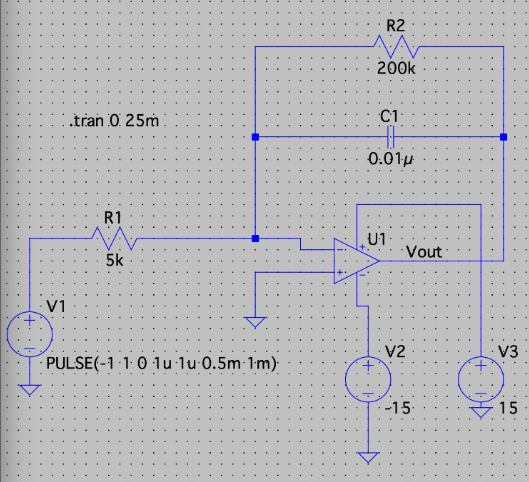
\includegraphics[scale=0.5]{pre_task1_circuit.png}
\end{center}
\caption{Integrator Circuit Diagram}
\end{figure}
}
% put task 1 result as welll

\noindent
The simulation result for the integrator circuit is shown below:

\begin{figure}[h]  
\begin{center}
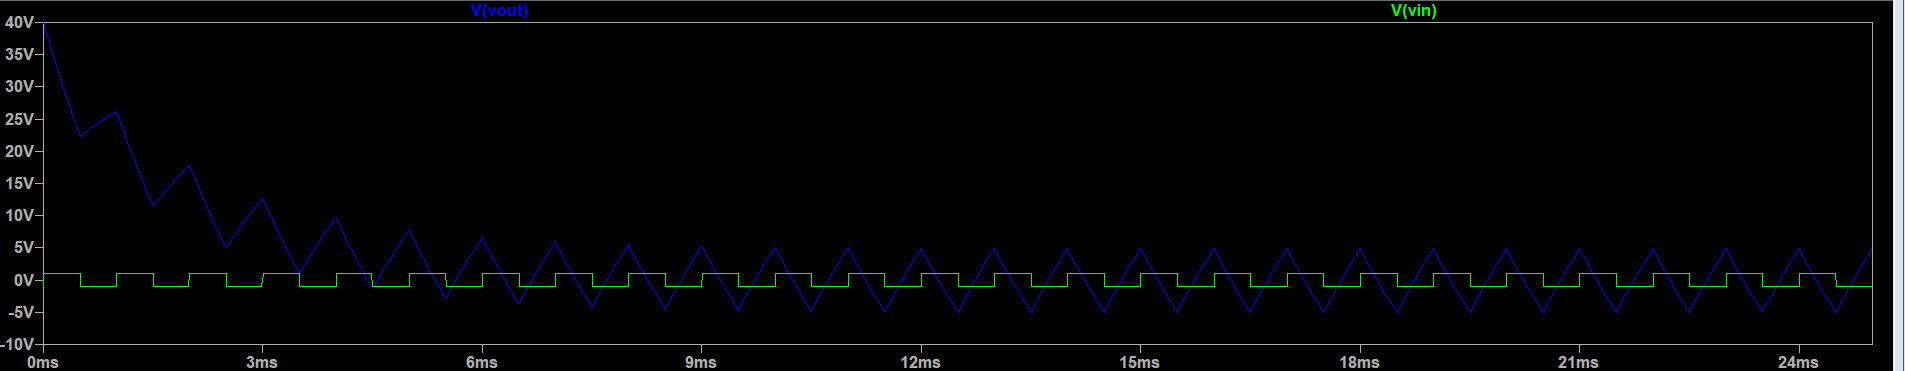
\includegraphics[scale=0.227]{pre_task1_result.png}
\end{center}
\caption{Simulation Result for Integrator Circuit}
\end{figure}

\noindent
\textbf{Comment:} The output of the practical integrator simulation begins at a high voltage and then stabilizes. Initial conditions like the voltage across the capacitor and small offset voltages in the op-amp are what generate this behavior. At first, these impacts produce a brief temporary. The output confirms proper operation as the circuit stabilizes by following the expected integral of the input signal.

\newpage
\subsubsection{Differentiator Circuit}
The differentiator circuit provided in the Lab Manual is simulated in LTSpice as shown below:
\begin{figure}[h]
\begin{center}
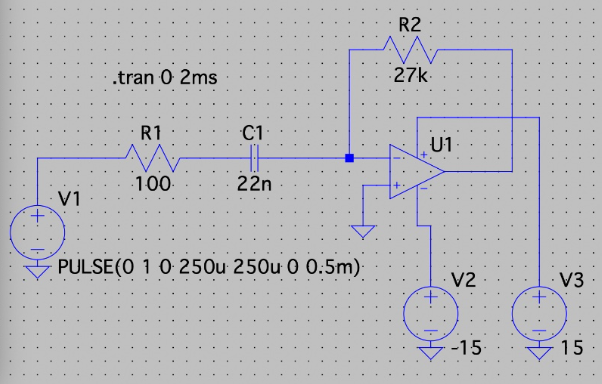
\includegraphics[scale=0.5]{pre_task2_circuit.png}
\end{center}
\caption{Differentiator Circuit Diagram.}
\end{figure}

\noindent
The simulation results for the differentiator circuit are shown below:
\begin{figure}[h]
\begin{center}
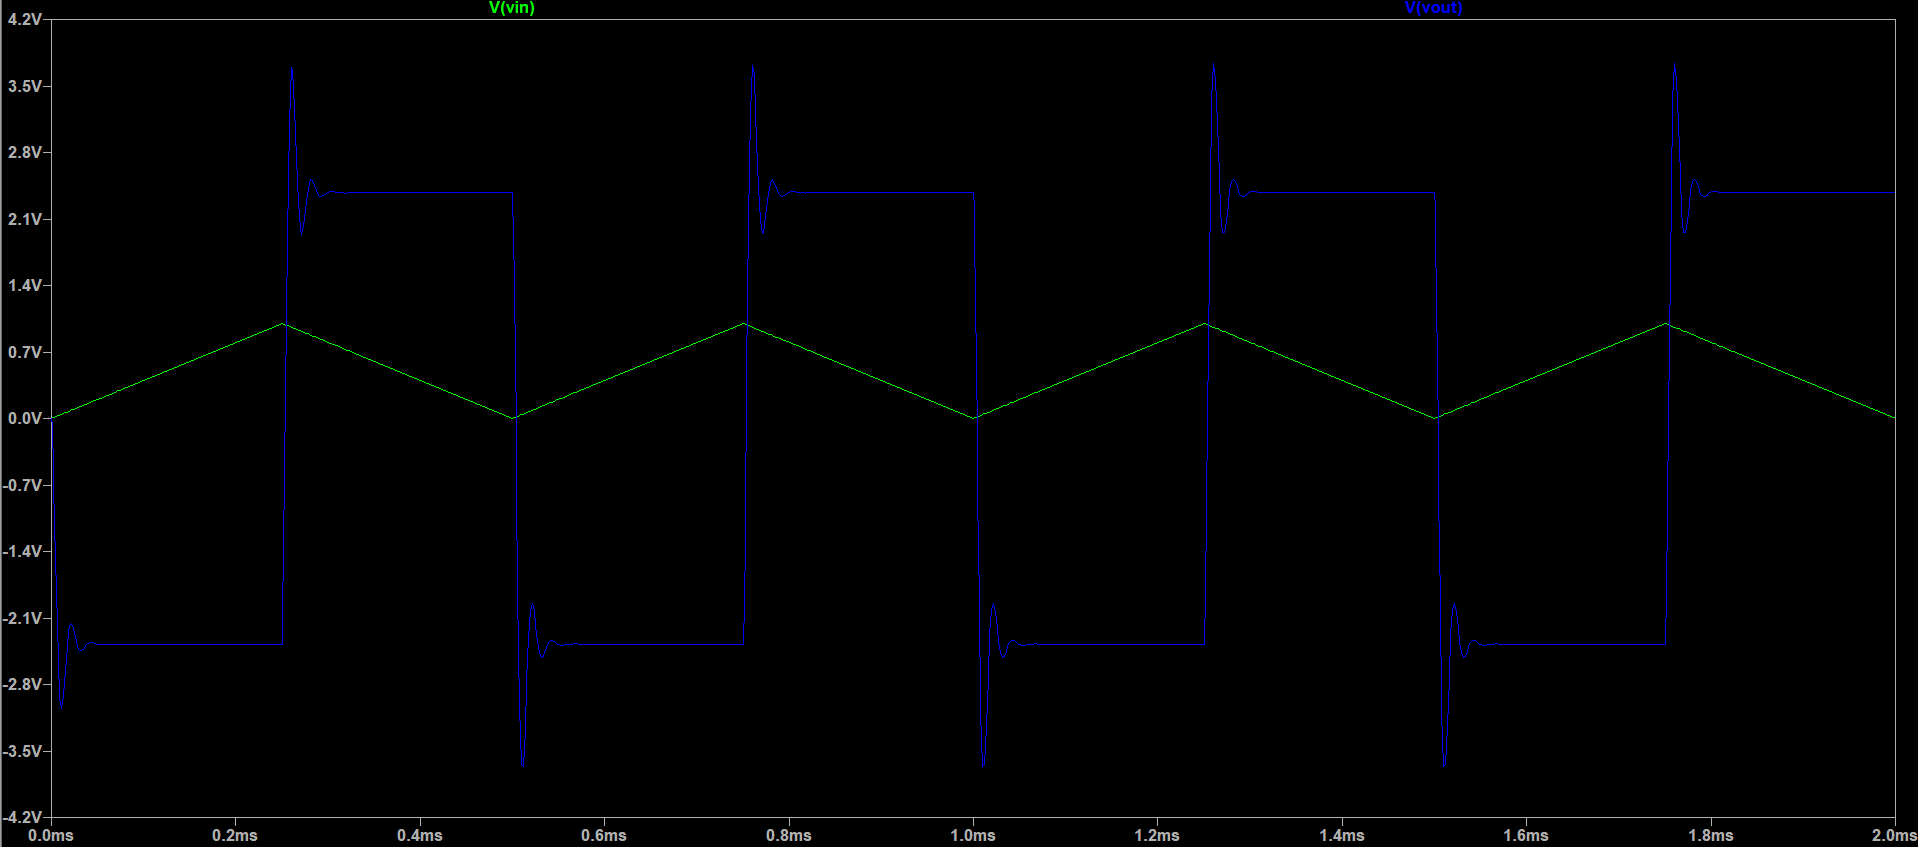
\includegraphics[scale=0.35]{pre_task2_result.png}
\end{center}
\caption{Simulation Result for Differentiator Circuit}
\end{figure}

\textbf{Comment:} For the differentiator circuit, the output reflects the derivative of the input ramp signal. Since the slope of a ramp is constant, the output remains steady during each segment. At the break point—where the ramp's slope changes—the derivative shifts abruptly, causing a sharp change in the output. This behavior matches the expected mathematical operation of a differentiator.

\newpage




































\subsection{Lab Tasks}

WRITE SOMETHIN HERE

\subsubsection{Task 1.}

The diagram shown in Figure 5 was built as shown in Figure 6 using a LM741 op-amp. After connecting ±15V power supply and grounding properly, the input was given from the signal generator.
\begin{figure}[h]
\begin{center}
\begin{minipage}{0.45\textwidth}
  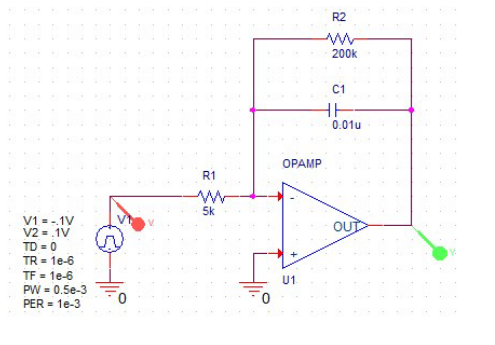
\includegraphics[width=\textwidth]{task1_diagram.png}
  \caption{Task 1 Circuit Diagram}
\end{minipage}
\hfill
\begin{minipage}{0.45\textwidth}
  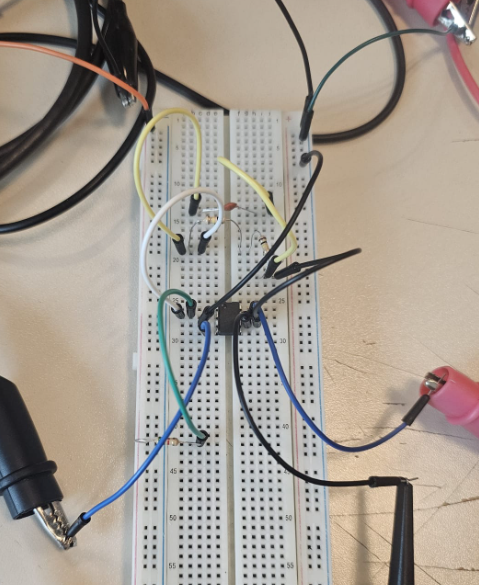
\includegraphics[width=\textwidth]{task1_circuit.png}
  \caption{Task 1 Simulation Result}
\end{minipage}
\end{center}
\end{figure}

\noindent
Different types of input waveforms and frequencies were applied to the circuit to observe its behavior. The results are shown in the following figures. In all cases, the yellow signal represents the input waveform, while the blue signal represents the corresponding output response. The circuit's response to square, triangular, and sinusoidal waves at varying frequencies demonstrates its functionality and highlights its frequency-dependent behavior.

\begin{itemize}
  
  \newpage
  \item \textbf{Applying 2kHz 0.1V Amplitude Square Wave}
  \begin{figure}[h]
    \begin{center}
      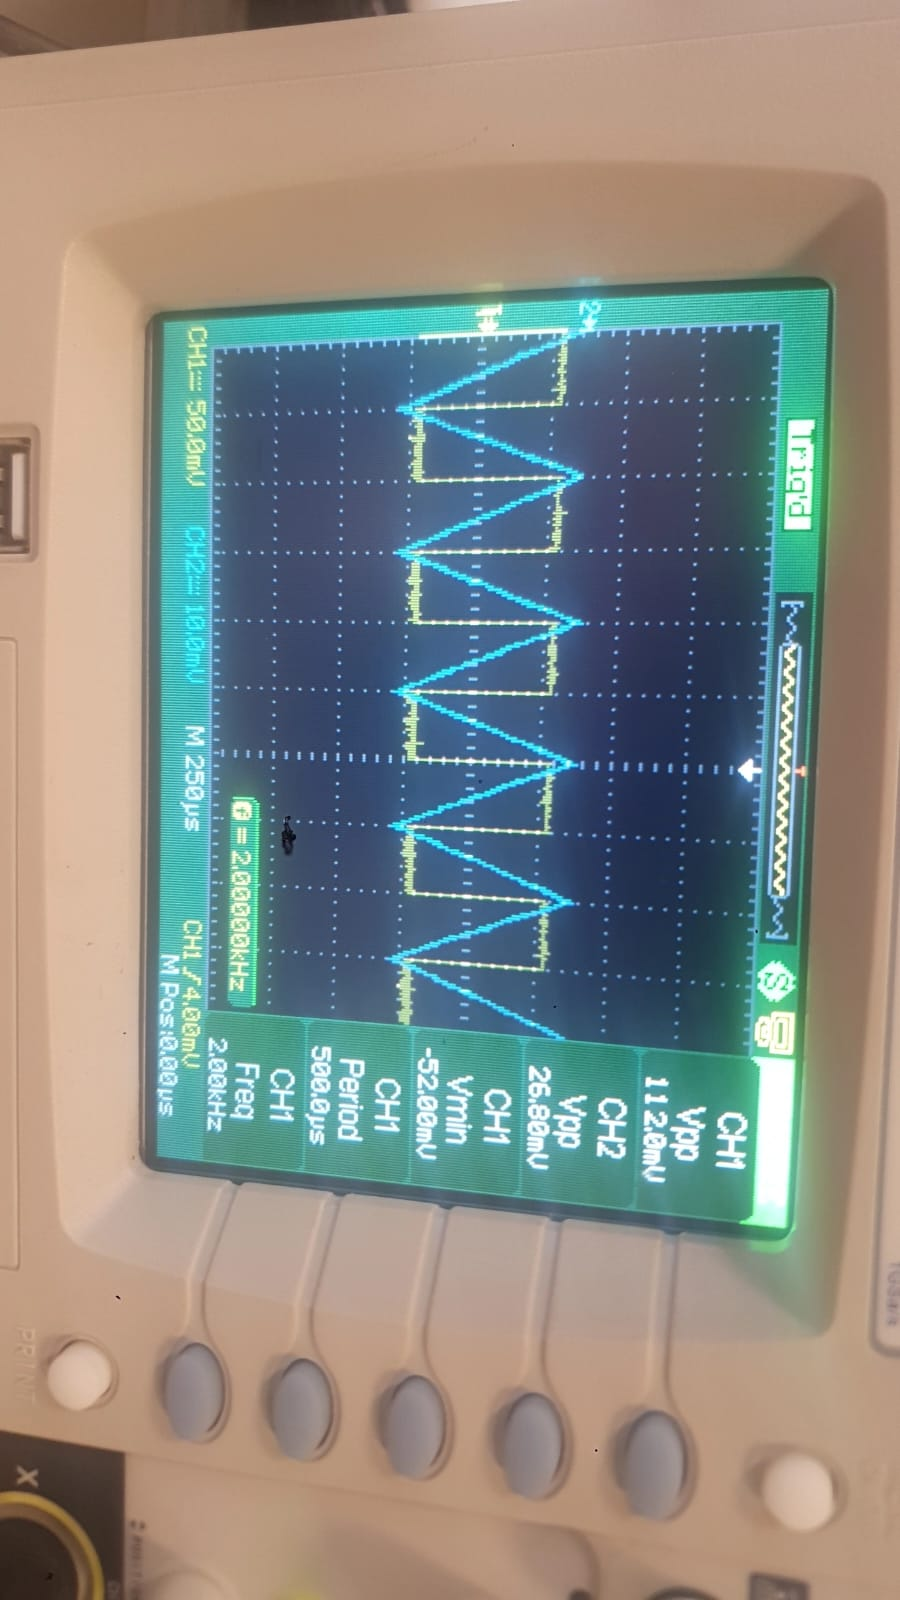
\includegraphics[scale=0.2, angle=90]{task1_square_wave.png}
      \caption{Square Wave Input Signal and Output Response}
    \end{center}
  \end{figure}  
  
  \item \textbf{Applying 2kHz 0.1 Amplitude Triangle Wave}
  \begin{figure}[h]
    \begin{center}
      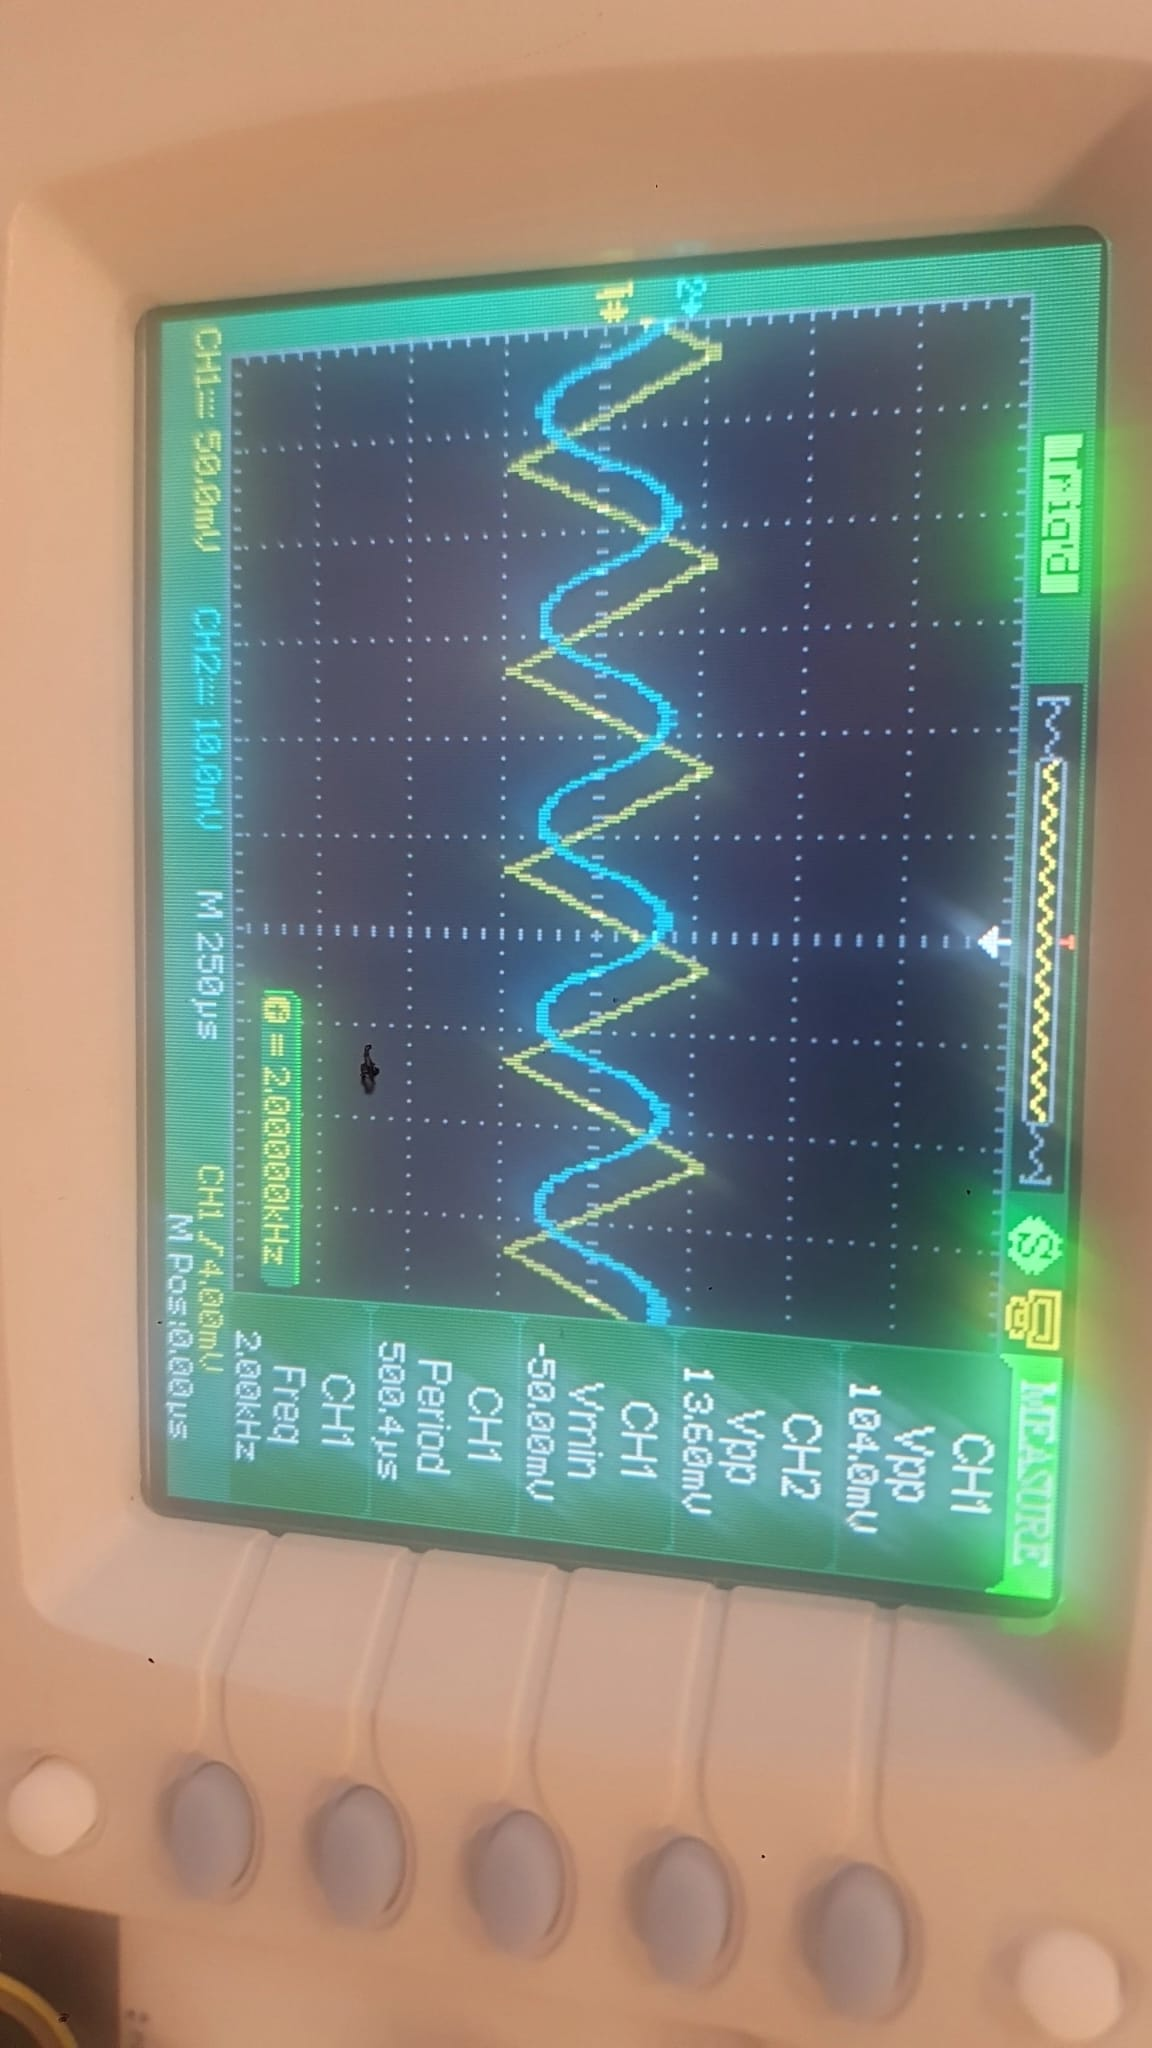
\includegraphics[scale=0.17, angle=90]{task1_triangle_wave.png}
      \caption{Triangle Wave Input Signal and Output Response}
    \end{center}
  \end{figure}  

  \newpage
  \item \textbf{Applying 1kHz 0.1V Amplitude Sinusoidal Wave}
  \begin{figure}[h]
    \begin{center}
      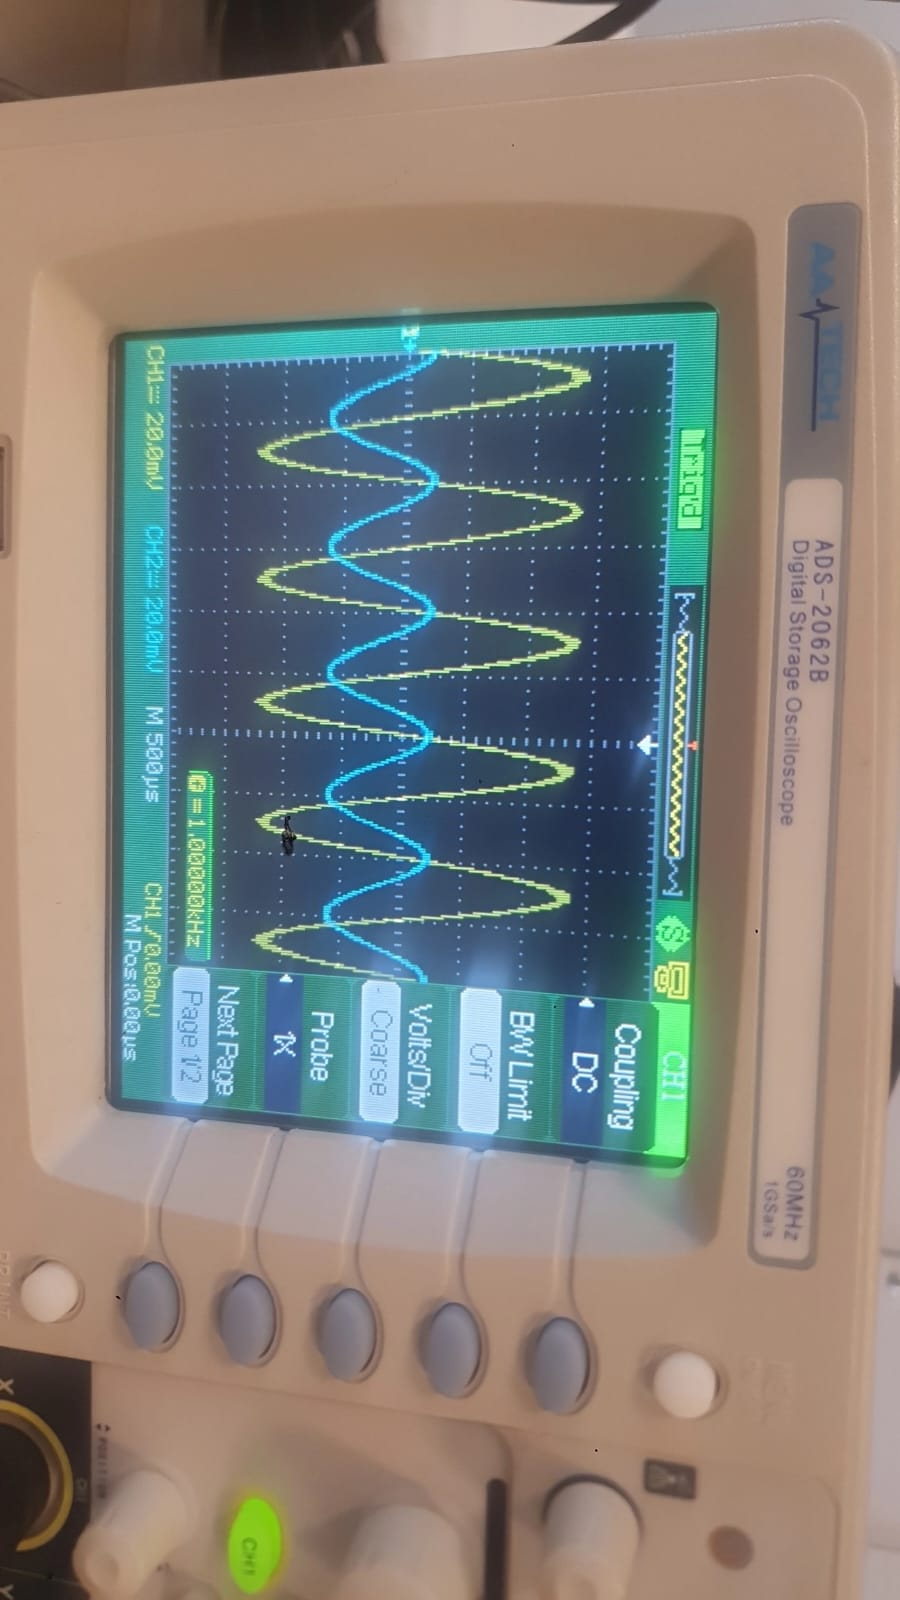
\includegraphics[scale=0.2, angle=90]{task1_sinusoidal_wave.png}
      \caption{Sinusoidal Wave Input Signal and Output Response}
    \end{center}
  \end{figure}
  

  \item \textbf{Applying 10kHz 0.1V Amplitude Sinusoidal Wave}
  
  \begin{figure}[h]
    \begin{center}
      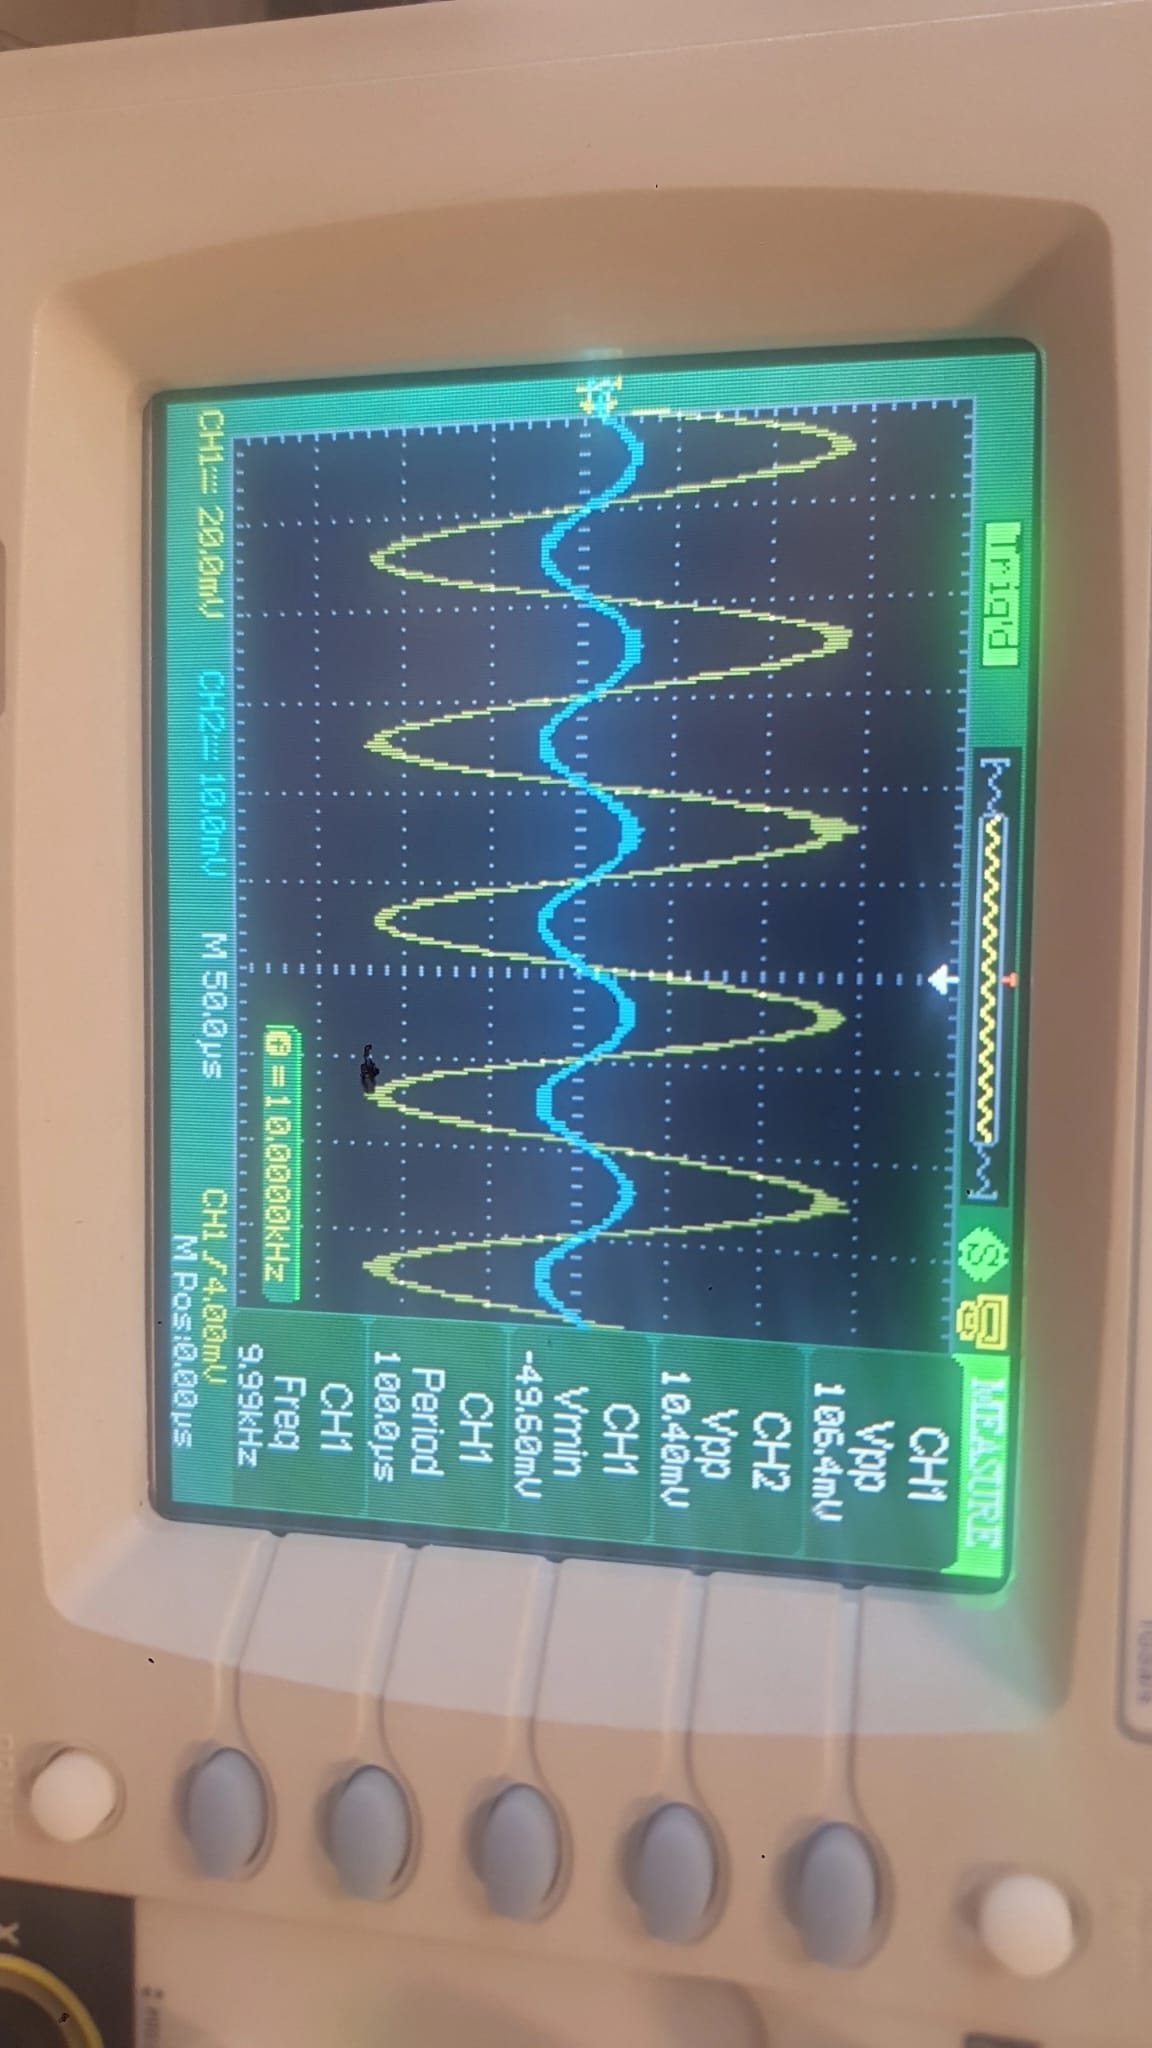
\includegraphics[scale=0.15, angle=90]{task1_10kHz_sinusoidal_wave.png}
      \caption{10kHz Sinusoidal Wave Input Signal and Output Response}
    \end{center}
  \end{figure}  

\end{itemize}

\newpage

\subsubsection{Task 2.}

The diagram shown in Figure 11 was built as shown in Figure 12 using a LM741 op-amp. Unlike Task 1, this circuit is configured as a differentiator, with different resistor and capacitor values. After connecting ±15V power supply and grounding properly, the input was given from the signal generator.

\begin{figure}[h]
\begin{center}
\begin{minipage}{0.45\textwidth}
  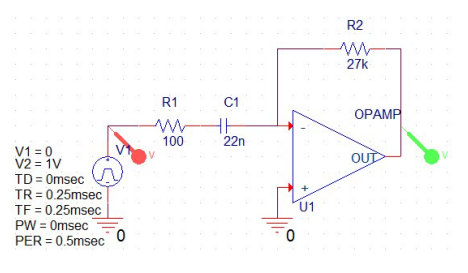
\includegraphics[width=\textwidth]{task2_diagram.png}
  \caption{Task 2 Circuit Diagram}
\end{minipage}
\hfill
\begin{minipage}{0.45\textwidth}
  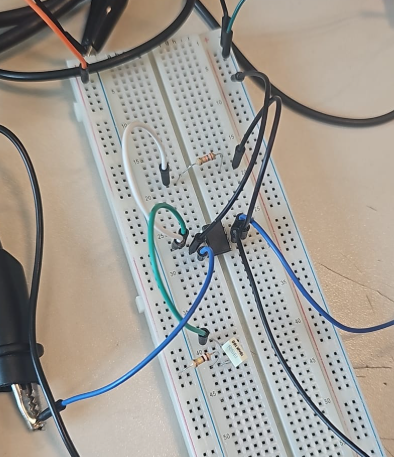
\includegraphics[width=\textwidth]{task2_circuit.png}
  \caption{Task 2 Simulation Result}
\end{minipage}
\end{center}
\end{figure}

\noindent
Similar to Task 1, different types of input waveforms and frequencies were applied to the circuit to observe its behavior. The results are shown in the following figures. In all cases, the yellow signal represents the input waveform, while the blue signal represents the corresponding output response. The circuit's response to triangular, sinusoidal waves at varying frequencies demonstrates its functionality as a differentiator and highlights its frequency-dependent behavior.

\begin{itemize}
  \item \textbf{Applying 2kHz 1V Amplitude Triangular Wave}
  \begin{figure}[h]
    
    \begin{center}
      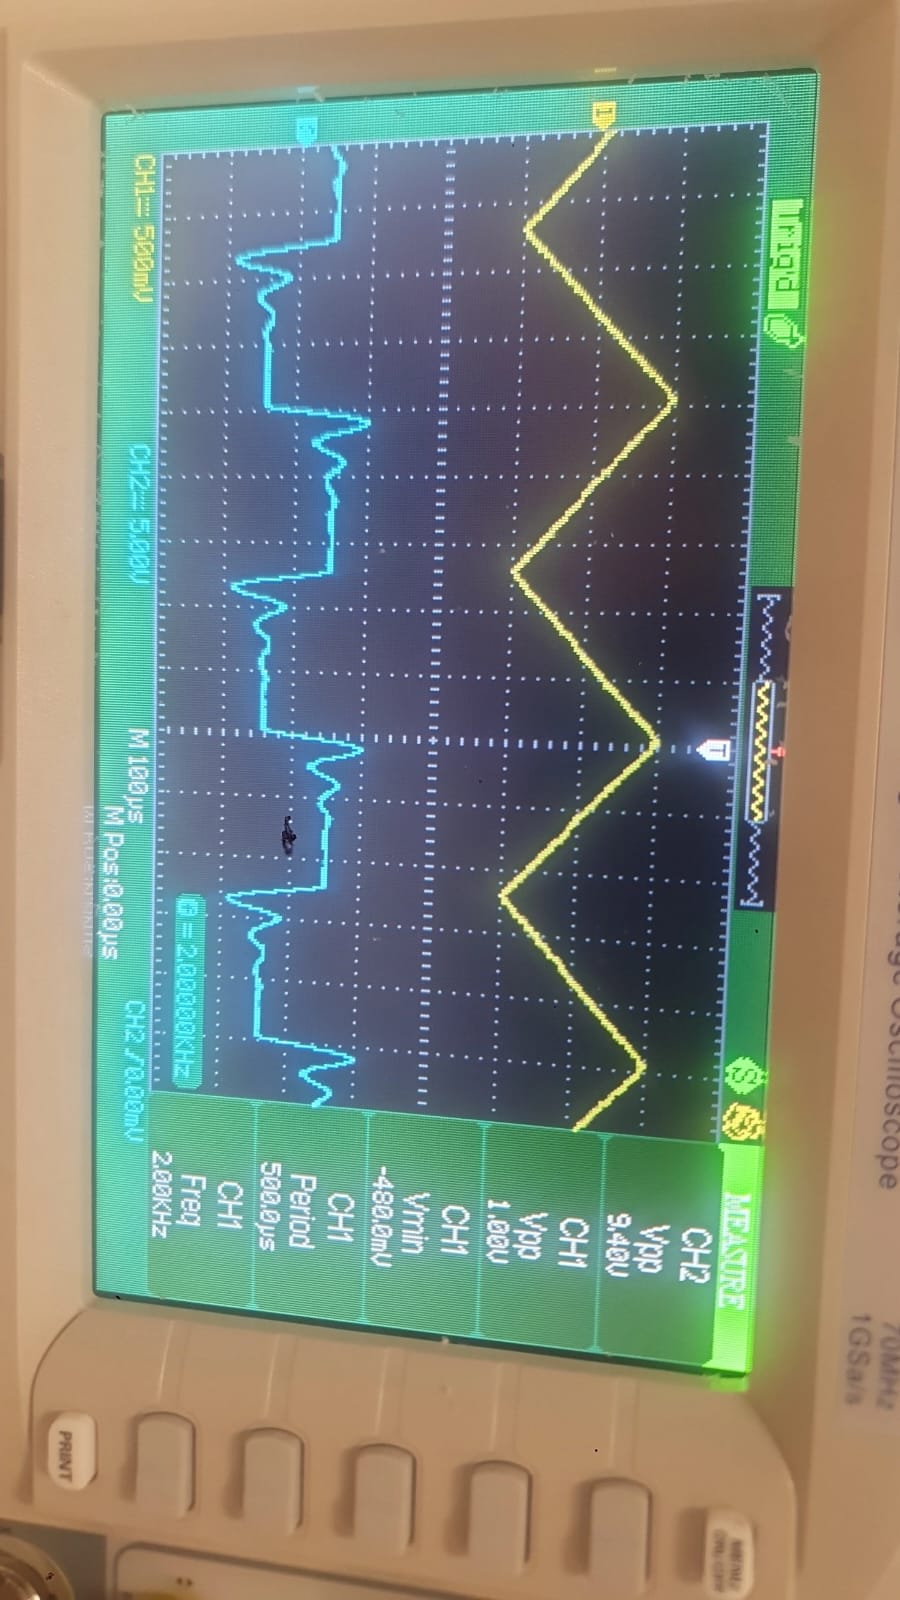
\includegraphics[scale=0.19, angle=90]{task2_triangular_wave.png}
      \caption{Triangular Wave Input Signal and Output Response}
    \end{center}
  \end{figure}

  \item \textbf{Applying 2kHz 1V Amplitude Square Wave}
  \begin{figure}[h]
    \begin{center}
      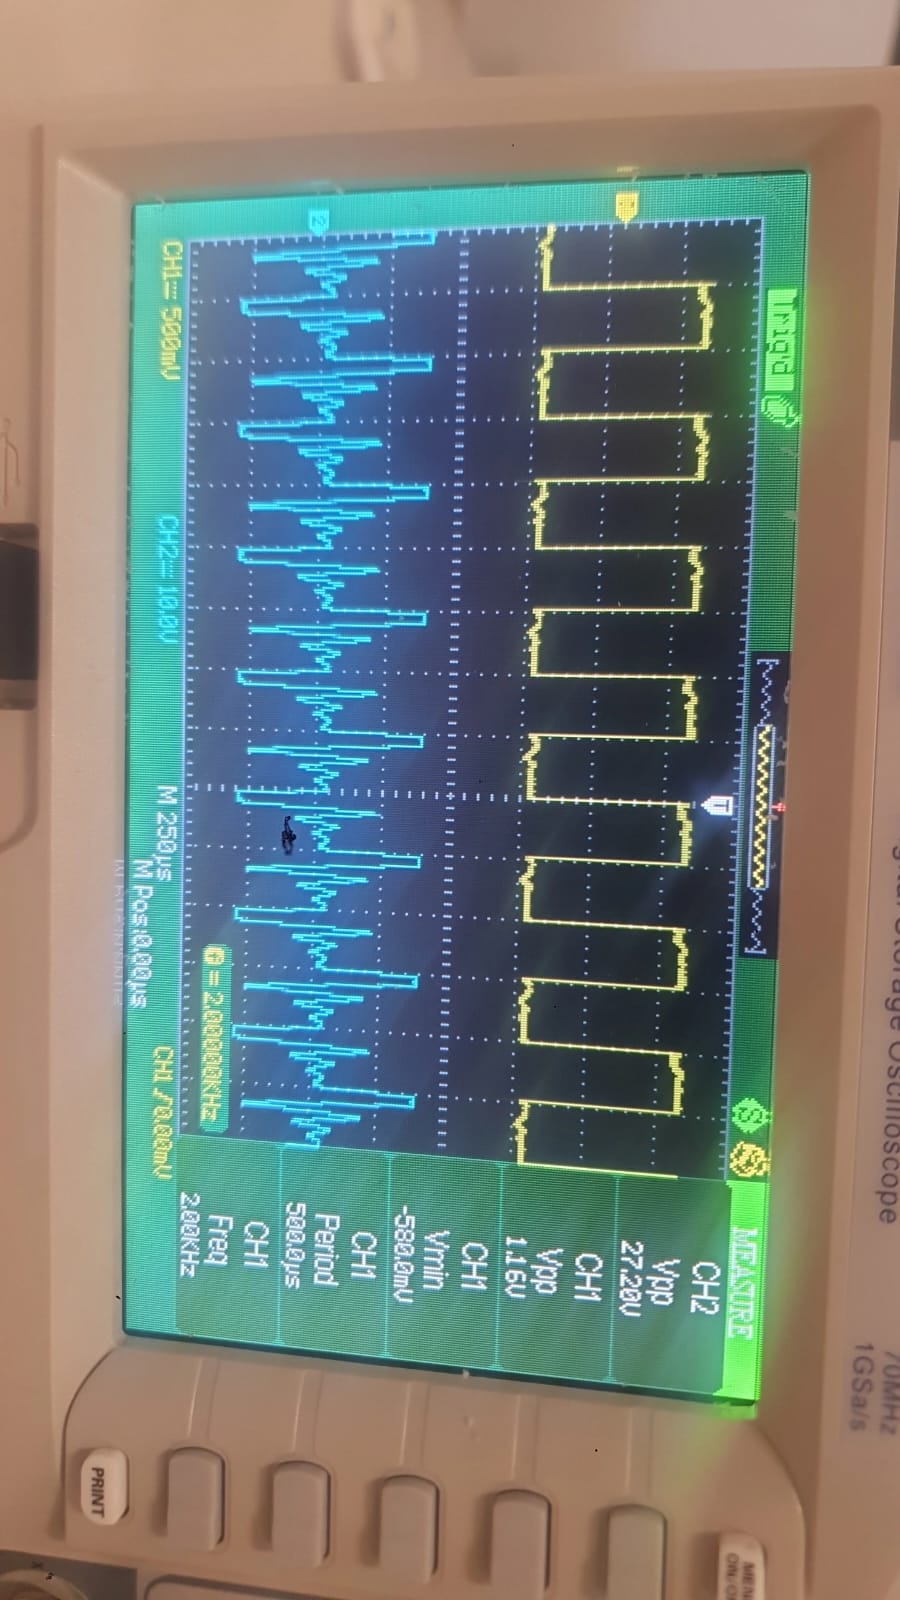
\includegraphics[scale=0.2, angle=90]{task2_square_wave.png}
      \caption{Square Wave Input Signal and Output Response}
    \end{center}
  \end{figure}

  \item \textbf{Applying 1kHz 1V Sinusoidal Wave}
  
  \begin{figure}[h]
    \begin{center}
      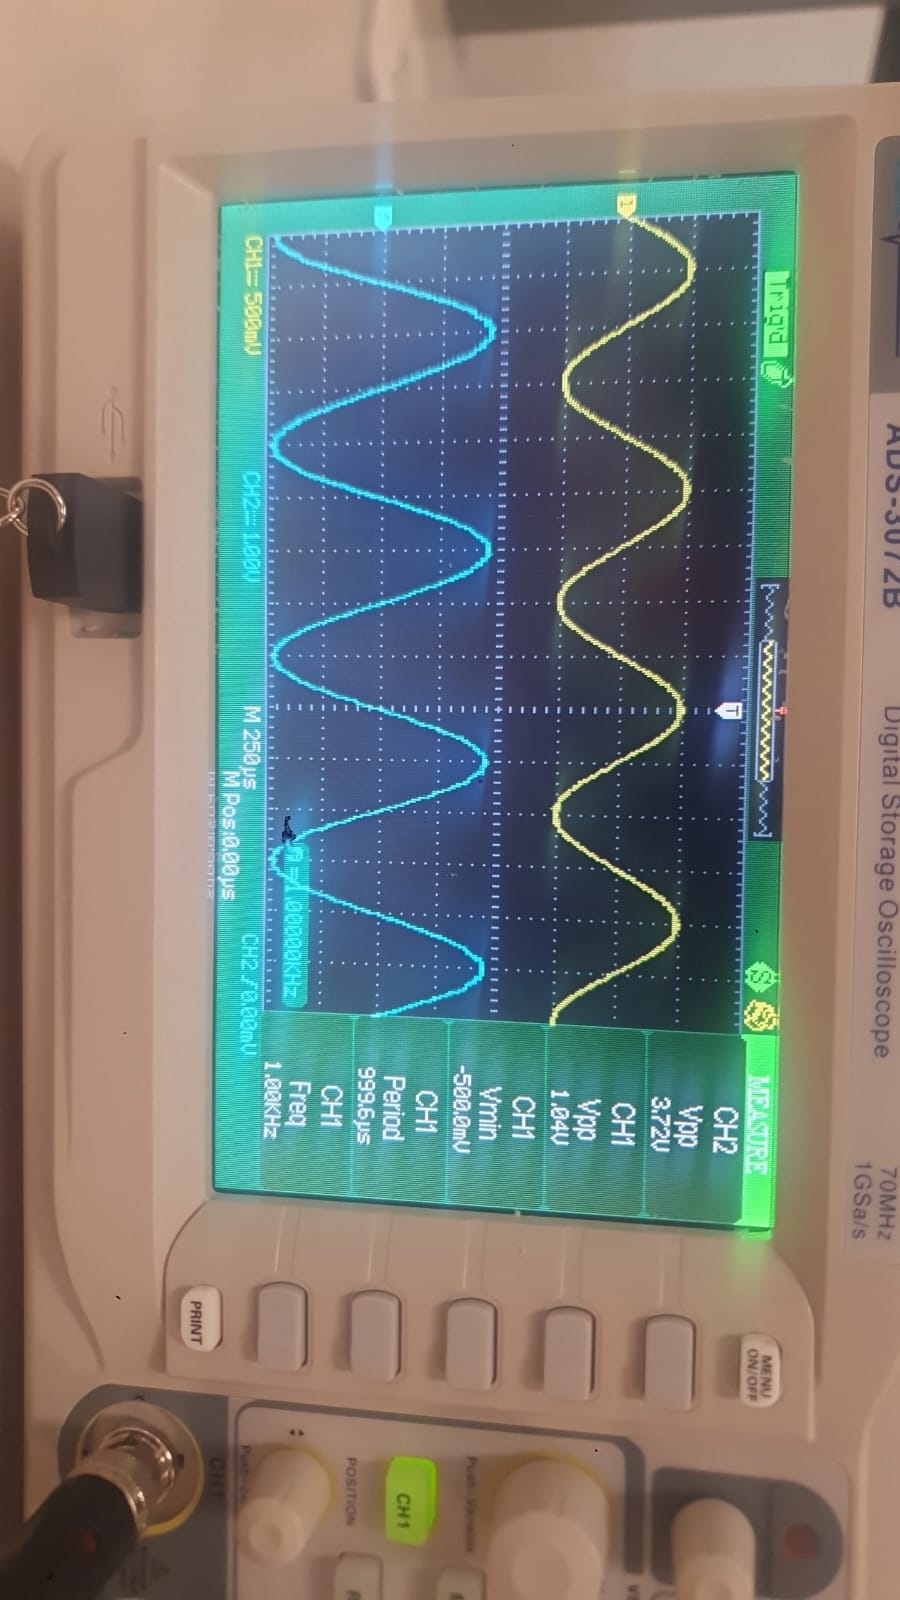
\includegraphics[scale=0.2, angle=90]{task2_1kHz_sinusoidal_wave.png}
      \caption{1kHz Sinusoidal Wave Input Signal and Output Response}
    \end{center}
  \end{figure}

  \newpage
  \item \textbf{Applying 10kHz 1V Sinusoidal Wave}
  
  \begin{figure}[h]
    \begin{center}
      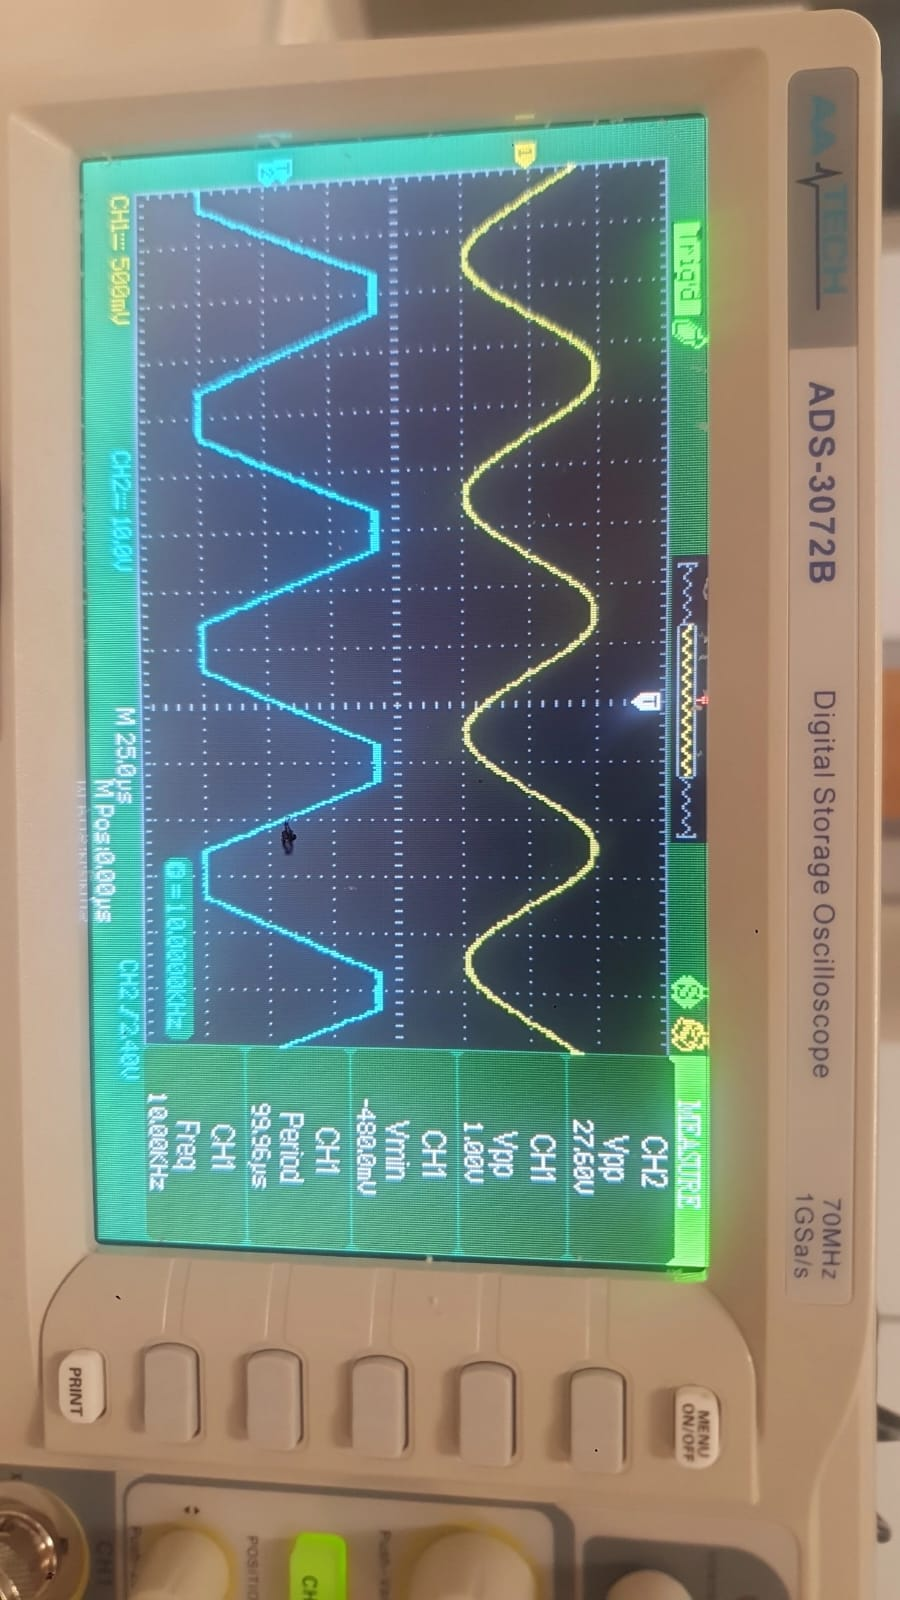
\includegraphics[scale=0.15, angle=90]{task2_10kHz_sinusoidal_wave.png}
      \caption{10kHz Sinusoidal Wave Input Signal and Output Response}
    \end{center}
  \end{figure}
  

\end{itemize}




\section{Conclusion}
\subsection{Task 1}
In this task, the integrator circuit was successfully built and tested using different input waveforms. The circuit behaved as expected, producing an output that represents the integral of the input signal. For example, when a square wave was applied, the output resembled a triangular waveform. Similarly, a sine wave input resulted in a cosine-like output, verifying the integration behavior. As the frequency increased, the output amplitude decreased, showing the frequency-dependent nature of the integrator. Overall, the results confirmed that the circuit performs the integration operation correctly.

\subsection{Task 2}
In Task 2, the differentiator circuit was constructed and tested with various input signals, including triangular, square, and sinusoidal waveforms. While the circuit performed its basic function of differentiating the input, the results were not always ideal. For example, the output for a square wave input showed high-frequency noise and ringing instead of clean impulses. At higher frequencies like 10kHz, the output exhibited clipping and distortion, likely due to the lack of a feedback capacitor and the op-amp’s tendency to amplify rapid transitions and noise. These effects highlight the practical limitations of real-world differentiator circuits. Despite these issues, the task successfully demonstrated the differentiator’s behavior.






\end{document}
